\section{Problem C}
\textit{For each of the channel realizations generated in (B) perform time reversal from a single antenna. Store the new equivalent channel impulse responses, with and without power normalization and the transmitter. Calculate the new power delay profile and from that the delay spread. How does it compare to the delay spread calculated in (B)?}

The code to perform this task is shown in the following code snippet 

\code{language=Matlab,caption = Time reversal operation,label=cl:imp_resp_code,linerange={74-146},firstnumber=74}{code/mm1/mm1_pretty_solution_pretty_coments_Labels_and_DB.m}

The resulting plots are shown in \figref{fig:ex_c_non_normalized} and \figref{fig:ex_c_normalized} for the non-normalized and normalized power.

\begin{figure}
\centering
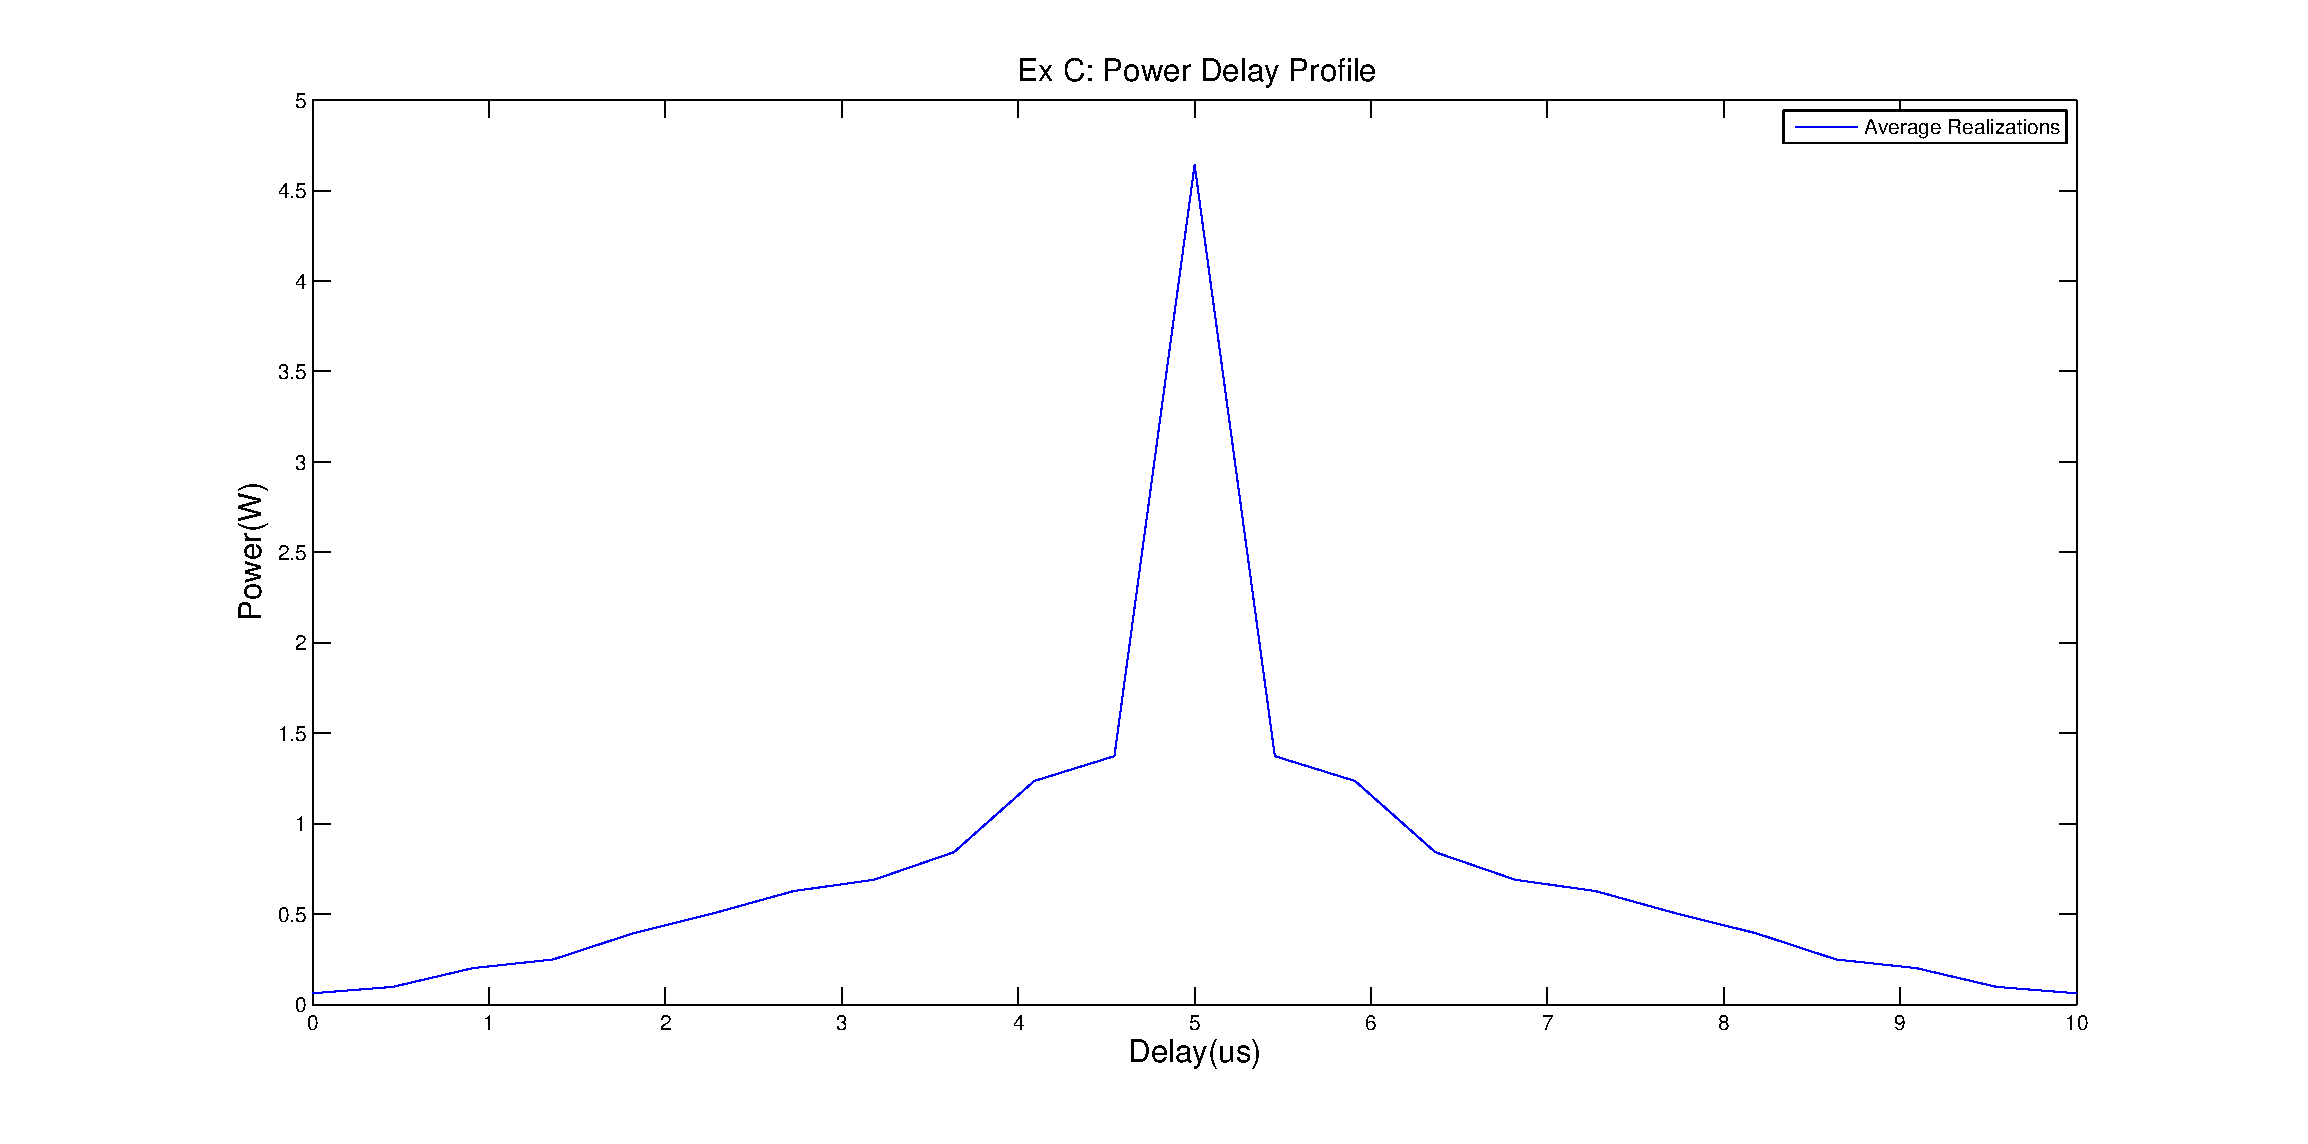
\includegraphics[width=9cm]{ex_c_non_normalized.eps}
\caption{PDP non normalized power}\label{fig:ex_c_non_normalized}
\end{figure}

\begin{figure}
\centering
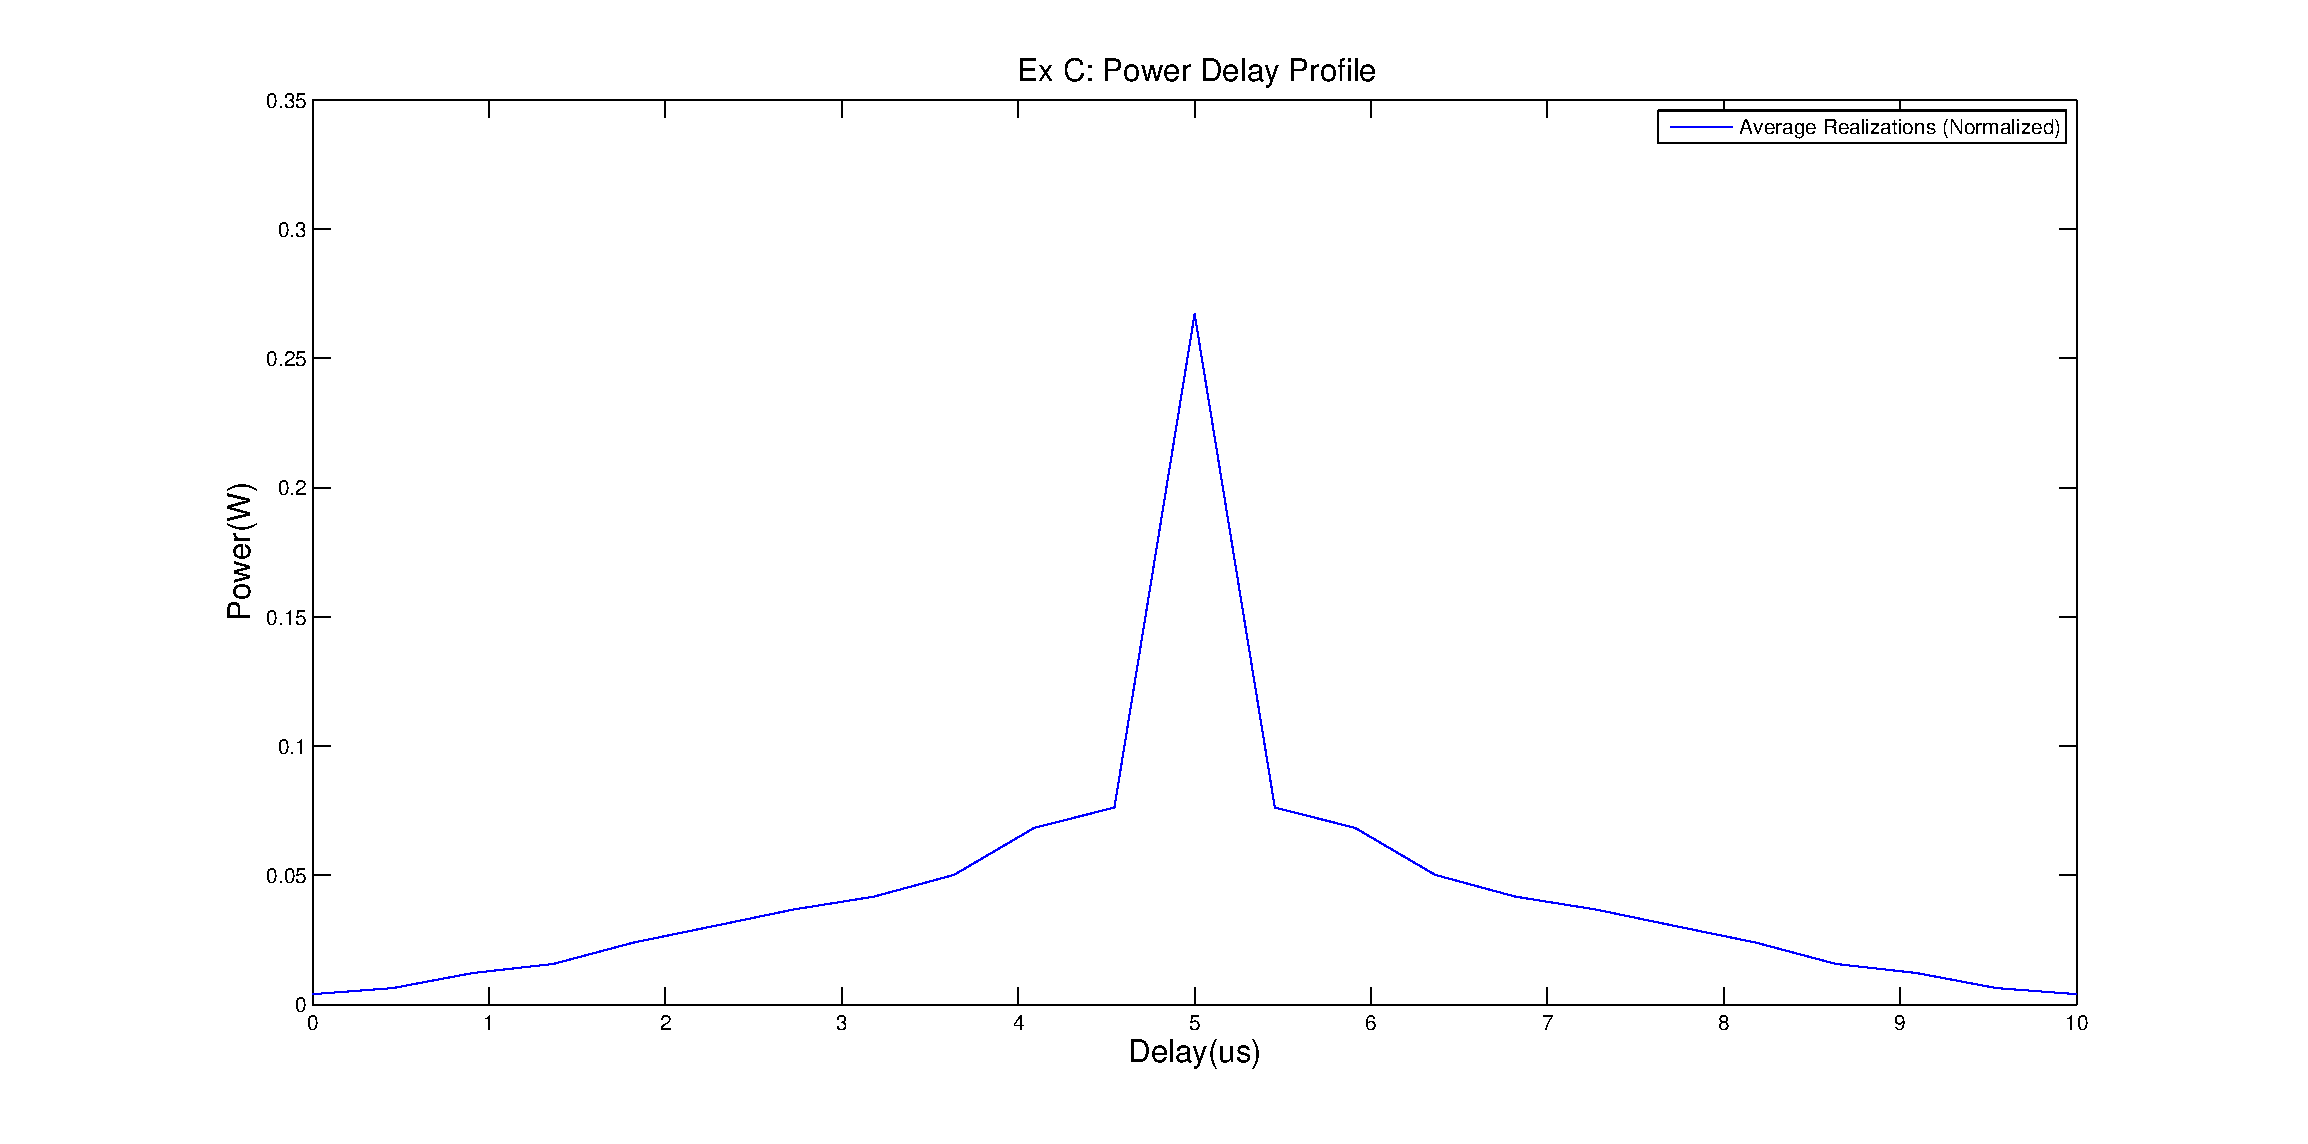
\includegraphics[width=9cm]{ex_c_normalized.eps}
\caption{PDP normalized power}\label{fig:ex_c_normalized}
\end{figure}

The delay spread of the time reversed signal is
\begin{flalign}
&& \sigma_{\text{ds}} =& \SI{1.753}{\micro\second} &
\end{flalign}

It can be seen from the plots and from the numerical value of the delay spread of the time reversed signal, that as expected, this signal is time expanded compared to the original signal. Mathematically this is due to the convolution operation.